\documentclass[tikz,border=5pt]{standalone}
\usepackage{tikz}
\usetikzlibrary{arrows.meta}
\begin{document}
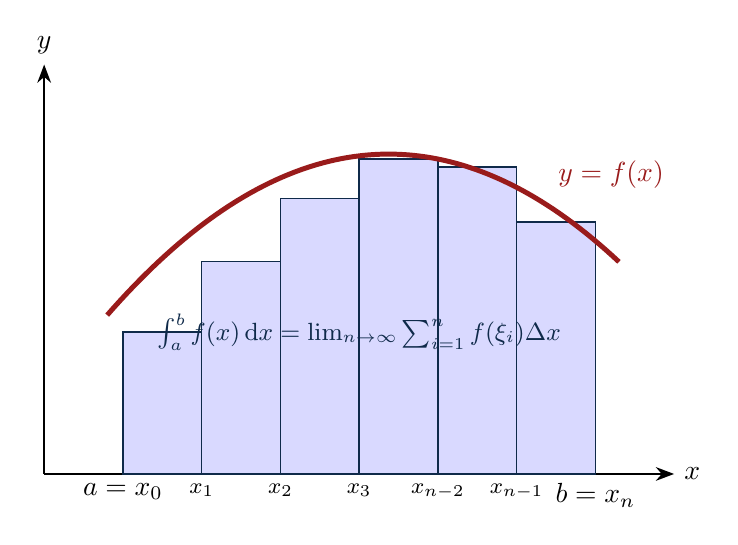
\begin{tikzpicture}[>=Stealth, scale=1.0]
  \definecolor{navyblue}{HTML}{0F2A4A}
  \definecolor{accentcrimson}{HTML}{991B1B}

  % Axes
  \draw[thick, ->] (0,0) -- (8.0,0) node[right, font=\sffamily\bfseries] {$x$};
  \draw[thick, ->] (0,0) -- (0,5.2) node[above, font=\sffamily\bfseries] {$y$};

  % Riemann Rectangles
  \fill[blue!15, draw=navyblue, line width=0.6pt] (1.0, 0) rectangle (2.0, 1.8);
  \fill[blue!15, draw=navyblue, line width=0.6pt] (2.0, 0) rectangle (3.0, 2.7);
  \fill[blue!15, draw=navyblue, line width=0.6pt] (3.0, 0) rectangle (4.0, 3.5);
  \fill[blue!15, draw=navyblue, line width=0.6pt] (4.0, 0) rectangle (5.0, 4.0);
  \fill[blue!15, draw=navyblue, line width=0.6pt] (5.0, 0) rectangle (6.0, 3.9);
  \fill[blue!15, draw=navyblue, line width=0.6pt] (6.0, 0) rectangle (7.0, 3.2);

  % Continuous curve
  \draw[line width=1.8pt, accentcrimson, domain=0.8:7.3, samples=80] 
    plot (\x, {1.0 + 1.4*\x - 0.16*\x*\x});
  \node[accentcrimson, font=\sffamily\bfseries] at (7.2, 3.8) {$y = f(x)$};

  % Labels
  \node[below, font=\sffamily\bfseries] at (1.0, 0) {$a = x_0$};
  \node[below, font=\sffamily\footnotesize] at (2.0, 0) {$x_1$};
  \node[below, font=\sffamily\footnotesize] at (3.0, 0) {$x_2$};
  \node[below, font=\sffamily\footnotesize] at (4.0, 0) {$x_3$};
  \node[below, font=\sffamily\footnotesize] at (5.0, 0) {$x_{n-2}$};
  \node[below, font=\sffamily\footnotesize] at (6.0, 0) {$x_{n-1}$};
  \node[below, font=\sffamily\bfseries] at (7.0, 0) {$b = x_n$};

  \node[font=\sffamily\small\bfseries, navyblue] at (4.0, 1.8) {$\int_a^b f(x)\,\mathrm{d}x = \lim_{n \to \infty} \sum_{i=1}^n f(\xi_i) \Delta x$};
\end{tikzpicture}
\end{document}